% Chapter 20: Deep Generative Models

\chapter{Deep Generative Models}
\label{chap:deep-generative-models}

This chapter examines modern approaches to generating new data samples using deep learning.


\begin{learningobjectives}
\objective{VAEs, GANs, and flow/diffusion models conceptually and practically}
\objective{Training objectives and sampling procedures for each class}
\objective{Generative models with proper metrics and qualitative checks}
\objective{Trade-offs in likelihood, sample quality, and mode coverage}
\end{learningobjectives}



\section*{Intuition}
\addcontentsline{toc}{section}{Intuition}

Generative models are machine learning systems that learn to create new data samples that resemble a given dataset. For example, after training on thousands of cat photos, a generative model can produce entirely new, realistic cat images that never existed before.

Think of generative models as digital artists who study masterpieces to understand artistic style, then create original works in that same style. Just as a painter learns brushstrokes and color palettes from studying great works, these models learn the underlying patterns and structures in data to generate novel samples.

Generative models learn data distributions in complementary ways: explicit likelihoods, implicit adversarial training, or score-based diffusion. Each chooses a tractable learning signal that captures structure while managing complexity.


% Chapter 20, Section 1

\section{Variational Autoencoders (VAEs) \difficultyInline{advanced}}
\label{sec:vaes}

(See also Chapter 14 for detailed VAE coverage.)

\subsection{Recap}

VAE learns latent representation $\vect{z}$ and decoder $p_{\theta}(\vect{x}|\vect{z})$:
\begin{equation}
\max_{\theta, \phi} \mathbb{E}_{q_{\phi}(\vect{z}|\vect{x})}[\log p_{\theta}(\vect{x}|\vect{z})] - D_{KL}(q_{\phi}(\vect{z}|\vect{x}) \| p(\vect{z}))
\end{equation}

The VAE objective consists of two terms: the reconstruction loss $\mathbb{E}_{q_{\phi}(\vect{z}|\vect{x})}[\log p_{\theta}(\vect{x}|\vect{z})]$ encourages the decoder to accurately reconstruct input data from latent codes, while the KL divergence term $D_{KL}(q_{\phi}(\vect{z}|\vect{x}) \| p(\vect{z}))$ regularizes the encoder to produce latent distributions close to the prior $p(\vect{z})$. This balance ensures both faithful reconstruction and meaningful latent representations.

\subsection{Conditional VAEs}

Generate conditioned on class or attributes:
\begin{equation}
\max \mathbb{E}_{q(\vect{z}|\vect{x}, y)}[\log p(\vect{x}|\vect{z}, y)] - D_{KL}(q(\vect{z}|\vect{x}, y) \| p(\vect{z}))
\end{equation}

Conditional VAEs extend the standard VAE framework by incorporating conditioning information $y$ (such as class labels or attributes) into both the encoder and decoder. The encoder $q(\vect{z}|\vect{x}, y)$ learns to map input data and conditioning information to latent codes, while the decoder $p(\vect{x}|\vect{z}, y)$ generates samples conditioned on both the latent code and the conditioning variable. This enables controlled generation of specific types of content.

\subsection{Disentangled Representations}

\textbf{$\beta$-VAE:} Increase KL weight for disentanglement
\begin{equation}
\mathcal{L} = \mathbb{E}_{q}[\log p(\vect{x}|\vect{z})] - \beta D_{KL}(q(\vect{z}|\vect{x}) \| p(\vect{z}))
\end{equation}

The $\beta$-VAE introduces a hyperparameter $\beta$ that controls the strength of the KL regularization term. When $\beta > 1$, the model is encouraged to learn more independent latent factors, where each dimension of $\vect{z}$ corresponds to a distinct, interpretable attribute of the data. This disentanglement is achieved by penalizing the mutual information between latent dimensions, forcing the model to encode different aspects of variation in separate latent variables.

% \subsection{Visual aids}
% \addcontentsline{toc}{subsubsection}{Visual aids (VAE recap)}

% \begin{figure}[h]
%   \centering
%   \begin{tikzpicture}
%     \begin{axis}[
%       width=0.48\textwidth,height=0.36\textwidth,
%       xlabel={$z_1$}, ylabel={$z_2$}, grid=both]
%       \addplot+[only marks,mark=*,mark size=0.9pt,bookpurple!70] coordinates{(-2,-2) (-1,0) (0,0) (1,1) (2,2)};
%     \end{axis}
%   \end{tikzpicture}
%   \caption{Latent samples from a learned VAE prior/posterior (illustrative).}
%   \label{fig:vae20-latent}
% \end{figure}

% \subsection{Notes and references}

% See \textcite{Kingma2013,GoodfellowEtAl2016,Prince2023} for VAE objectives, conditional VAEs, and disentanglement.


% Chapter 20, Section 2

\section{Generative Adversarial Networks (GANs) \difficultyInline{advanced}}
\label{sec:gans}

GANs train two competing neural networks—a generator that creates fake data and a discriminator that tries to detect the fakes—in an adversarial game that eventually produces highly realistic synthetic samples.

\subsection{Core Idea}

The fundamental concept behind GANs is elegantly simple yet powerful. Imagine an art forger trying to create paintings so convincing that even expert art critics cannot distinguish them from genuine masterpieces. The forger (generator) continuously improves their technique based on feedback from the critics (discriminator), while the critics become more sophisticated at detecting fakes. This adversarial relationship drives both parties to become increasingly skilled—the forger learns to create more realistic art, while the critics develop sharper detection abilities.

In the GAN framework, the generator $G$ takes random noise as input and transforms it into synthetic data samples that should be indistinguishable from real data. The discriminator $D$ acts as a binary classifier, receiving both real and generated samples and learning to distinguish between them. As training progresses, the generator becomes increasingly adept at fooling the discriminator, while the discriminator becomes better at detecting subtle differences between real and fake samples.

\begin{figure}[h]
  \centering
  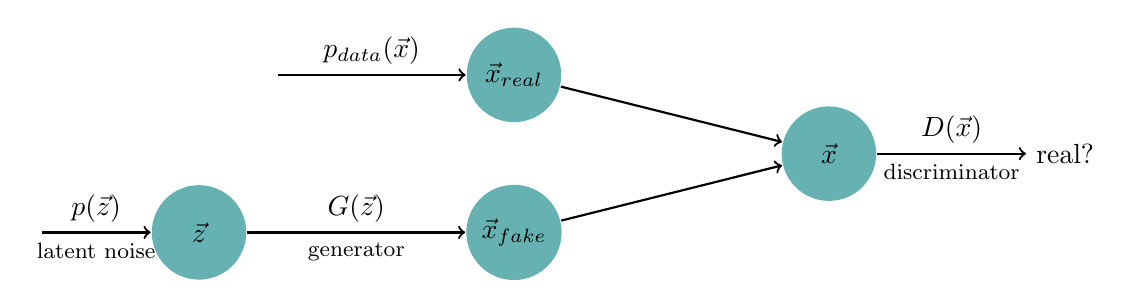
\begin{tikzpicture}[
    ->, thick,
    node/.style={circle, fill=teal!60, minimum size=1.2cm},
    label/.style={below, font=\footnotesize},
  ]

  % Generator path
  \node[node] (zin) at (0,0) {$\vec z$};
  \node[node] (fake) at (4,0) {$\vec x_\text{fake}$};
  \draw (zin) -- node[above] {$G(\vec z)$} node[label] {generator} (fake);

  % Real data path
  \node[node] (real) at (4,2) {$\vec x_\text{real}$};
  \draw[<-] (real) -- node[above] {$p_\text{data}(\vec x)$} ++(-3,0);

  % Discriminator
  \node[node] (D) at (8,1) {$\vec x$};
  \node (out) at (11,1) {real?};
  \draw (D) -- node[above] {$D(\vec x)$} node[label] {discriminator} (out);

  % Connections to discriminator
  \draw (fake) -- (D);
  \draw (real) -- (D);

  % Noise source
  \draw[<-] (zin) -- node[above] {$p(\vec z)$} node[label] {latent noise} ++(-2,0);

\end{tikzpicture}
\caption{GAN architecture showing the adversarial relationship between generator and discriminator.}
\label{fig:gan-architecture}
\end{figure}

\subsection{Objective}

Minimax game:
\begin{equation}
\min_G \max_D \mathbb{E}_{\vect{x} \sim p_{\text{data}}}[\log D(\vect{x})] + \mathbb{E}_{\vect{z} \sim p(\vect{z})}[\log(1 - D(G(\vect{z})))]
\end{equation}

The GAN objective represents a minimax game where the discriminator aims to maximize its ability to distinguish real from fake samples, while the generator seeks to minimize the discriminator's accuracy. The first term $\mathbb{E}_{\vect{x} \sim p_{\text{data}}}[\log D(\vect{x})]$ encourages the discriminator to assign high probability to real samples, while the second term $\mathbb{E}_{\vect{z} \sim p(\vect{z})}[\log(1 - D(G(\vect{z})))]$ penalizes the discriminator for correctly identifying generated samples, simultaneously training the generator to produce more convincing fakes.

\subsection{Training Procedure}

The training process alternates between updating the discriminator and generator in a carefully orchestrated dance. During each training iteration, the discriminator is first updated to improve its ability to distinguish real from fake samples. This involves maximizing the objective $\max_D \mathbb{E}_{\vect{x}}[\log D(\vect{x})] + \mathbb{E}_{\vect{z}}[\log(1 - D(G(\vect{z})))]$, which simultaneously rewards correct identification of real samples and penalizes misclassification of generated samples.

Following the discriminator update, the generator is trained to produce samples that are more likely to fool the updated discriminator. The generator's objective $\min_G \mathbb{E}_{\vect{z}}[\log(1 - D(G(\vect{z})))]$ encourages it to generate samples that the discriminator will classify as real. This alternating optimization process continues until the generator produces samples that are indistinguishable from real data, at which point the discriminator can no longer provide meaningful gradients for further improvement.

\subsection{Training Challenges}

GAN training presents several formidable challenges that can derail the delicate balance between generator and discriminator. Mode collapse occurs when the generator discovers a small subset of samples that consistently fool the discriminator, causing it to generate only these limited variations rather than exploring the full diversity of the data distribution. This phenomenon is particularly problematic when the discriminator becomes too strong relative to the generator, creating a feedback loop where the generator finds it easier to repeatedly generate the same convincing samples rather than learning the full data manifold.

Training instability manifests as oscillatory behavior where the generator and discriminator continuously outmaneuver each other without reaching a stable equilibrium. The discriminator may become too powerful, providing vanishing gradients to the generator, or the generator may become too skilled, causing the discriminator to lose its ability to provide meaningful learning signals. This instability often leads to non-convergence, where the training process fails to reach a meaningful solution despite extensive optimization efforts.

\subsection{GAN Variants}

The evolution of GAN architectures has addressed many of the fundamental challenges in adversarial training through innovative design choices and theoretical insights. DCGAN introduced architectural guidelines that stabilized training by using strided convolutions, batch normalization, and ReLU activations, establishing a foundation for successful deep convolutional GANs. WGAN revolutionized the field by replacing the Jensen-Shannon divergence with the Wasserstein distance, providing more stable gradients and better convergence properties that significantly reduced training instability.

StyleGAN represents a breakthrough in high-quality image generation by introducing a style-based generator architecture that separates high-level attributes from stochastic variation, enabling fine-grained control over generated images. Conditional GANs extend the basic framework by incorporating auxiliary information such as class labels, allowing for controlled generation of specific types of content. CycleGAN addresses the challenge of unpaired image-to-image translation by introducing cycle consistency constraints, enabling style transfer between domains without requiring paired training data.

% \subsection{Visual aids}
% \addcontentsline{toc}{subsubsection}{Visual aids (GANs)}

% \begin{figure}[h]
%   \centering
%   \begin{tikzpicture}[>=stealth]
%     \tikzstyle{b}=[draw,rounded corners,align=center,minimum width=2.4cm,minimum height=1.0cm]
%     \node[b,fill=bookpurple!10] at (0,0) (z) {Noise $\vect{z}$};
%     \node[b,fill=bookpurple!15] at (3.2,0) (g) {Generator $G$};
%     \node[b,fill=bookpurple!10] at (6.4,0.9) (x) {Real $\vect{x}$};
%     \node[b,fill=bookpurple!10] at (6.4,-0.9) (gx) {$G(\vect{z})$};
%     \node[b,fill=bookpurple!20] at (9.6,0) (d) {Discriminator $D$};
%     \draw[->] (z) -- (g);
%     \draw[->] (g) -- (gx);
%     \draw[->] (x) -- (d);
%     \draw[->] (gx) -- (d);
%   \end{tikzpicture}
%   \caption{GAN training: generator produces samples to fool discriminator.}
%   \label{fig:gan-diagram}
% \end{figure}

% \subsection{Notes and references}

% See \textcite{Goodfellow2014,GoodfellowEtAl2016,Prince2023} for GAN fundamentals and variants.


% Chapter 20, Section 3

\section{Normalizing Flows \difficultyInline{advanced}}
\label{sec:normalizing-flows}

\subsection{Key Idea}

Transform simple distribution (e.g., Gaussian) through invertible mappings:
\begin{equation}
\vect{x} = f_{\theta}(\vect{z}), \quad \vect{z} \sim p_z(\vect{z})
\end{equation}

\subsection{Change of Variables}

Density transforms as:
\begin{equation}
p_x(\vect{x}) = p_z(f^{-1}(\vect{x})) \left|\det \frac{\partial f^{-1}}{\partial \vect{x}}\right|
\end{equation}

or equivalently:
\begin{equation}
\log p_x(\vect{x}) = \log p_z(\vect{z}) - \log\left|\det \frac{\partial f}{\partial \vect{z}}\right|
\end{equation}

\subsection{Requirements}

Function $f$ must be:
\begin{itemize}
    \item Invertible
    \item Have tractable Jacobian determinant
\end{itemize}

\subsection{Flow Architectures}

\textbf{Coupling layers:} Split dimensions and transform half conditioned on other half

\textbf{Autoregressive flows:} Each dimension depends on previous ones

\textbf{Continuous normalizing flows:} Use neural ODEs

\subsection{Advantages}

\begin{itemize}
    \item Exact likelihood computation
    \item Exact sampling
    \item Stable training (no adversarial dynamics)
\end{itemize}

% \subsection{Visual aids}
% \addcontentsline{toc}{subsubsection}{Visual aids (flows)}

% \begin{figure}[h]
%   \centering
%   \begin{tikzpicture}
%     \begin{axis}[
%       width=0.48\textwidth,height=0.36\textwidth,
%       xlabel={$z_1$}, ylabel={$z_2$}, grid=both]
%       \addplot+[only marks,mark=*,mark size=0.8pt,bookpurple!60] coordinates{(-1,-1) (-1,1) (1,-1) (1,1)};
%     \end{axis}
%   \end{tikzpicture}
%   \caption{Toy latent samples before/after flow transformation (illustrative).}
%   \label{fig:flow-toy}
% \end{figure}

% \subsection{Notes and references}

% See \textcite{GoodfellowEtAl2016,Prince2023} for flow-based modeling and practical design choices.


% Chapter 20, Section 4

\section{Diffusion Models \difficultyInline{advanced}}
\label{sec:diffusion-models}

\subsection{Forward Process}

Gradually add noise over $T$ steps:
\begin{equation}
q(\vect{x}_t|\vect{x}_{t-1}) = \mathcal{N}(\vect{x}_t; \sqrt{1-\beta_t} \vect{x}_{t-1}, \beta_t \mat{I})
\end{equation}

Eventually $\vect{x}_T \approx \mathcal{N}(\boldsymbol{0}, \mat{I})$.

\subsection{Reverse Process}

Learn to denoise (reverse diffusion):
\begin{equation}
p_{\theta}(\vect{x}_{t-1}|\vect{x}_t) = \mathcal{N}(\vect{x}_{t-1}; \boldsymbol{\mu}_{\theta}(\vect{x}_t, t), \boldsymbol{\Sigma}_{\theta}(\vect{x}_t, t))
\end{equation}

\subsection{Training}

Predict noise $\boldsymbol{\epsilon}_{\theta}(\vect{x}_t, t)$ at each step:
\begin{equation}
\mathcal{L} = \mathbb{E}_{t, \vect{x}_0, \boldsymbol{\epsilon}}\left[\|\boldsymbol{\epsilon} - \boldsymbol{\epsilon}_{\theta}(\vect{x}_t, t)\|^2\right]
\end{equation}

\subsection{Sampling}

Start from noise and iteratively denoise:
\begin{equation}
\vect{x}_{t-1} = \frac{1}{\sqrt{\alpha_t}}\left(\vect{x}_t - \frac{1-\alpha_t}{\sqrt{1-\bar{\alpha}_t}}\boldsymbol{\epsilon}_{\theta}(\vect{x}_t, t)\right) + \sigma_t \vect{z}
\end{equation}

\subsection{Advantages}

\begin{itemize}
    \item High-quality generation (DALL-E 2, Stable Diffusion, Midjourney)
    \item Stable training
    \item Strong theoretical foundations
    \item Can condition on text, images, etc.
\end{itemize}

% \subsection{Visual aids}
% \addcontentsline{toc}{subsubsection}{Visual aids (diffusion)}

% \begin{figure}[h]
%   \centering
%   \begin{tikzpicture}
%     \begin{axis}[
%       width=0.48\textwidth,height=0.36\textwidth,
%       xlabel={Step $t$}, ylabel={Noise level}, grid=both]
%       \addplot[bookpurple,very thick] coordinates{(0,0.0) (10,0.2) (20,0.4) (30,0.6) (40,0.8) (50,1.0)};
%       \addplot[bookred,very thick,dashed] coordinates{(50,1.0) (40,0.8) (30,0.6) (20,0.4) (10,0.2) (0,0.0)};
%     \end{axis}
%   \end{tikzpicture}
%   \caption{Forward (solid) and reverse (dashed) diffusion noise schedules (illustrative).}
%   \label{fig:diffusion-schedule}
% \end{figure}

% \subsection{Notes and references}

% See \textcite{Ho2020,Prince2023} for DDPM training and sampling.


% Chapter 20, Section 5

\section{Applications and Future Directions \difficultyInline{advanced}}
\label{sec:generative-applications}

\subsection{Current Applications}

\textbf{Image generation:}
\begin{itemize}
    \item Text-to-image (DALL-E, Stable Diffusion)
    \item Image editing and inpainting
    \item Super-resolution
    \item Style transfer
\end{itemize}

\textbf{Text generation:}
\begin{itemize}
    \item Large language models (GPT family)
    \item Code generation
    \item Creative writing
\end{itemize}

\textbf{Audio/speech:}
\begin{itemize}
    \item Text-to-speech
    \item Music generation
    \item Voice conversion
\end{itemize}

\textbf{Video:}
\begin{itemize}
    \item Video prediction
    \item Video synthesis
    \item Animation
\end{itemize}

\textbf{Scientific applications:}
\begin{itemize}
    \item Molecule design
    \item Protein structure prediction
    \item Materials discovery
\end{itemize}

\subsection{Future Directions}

\begin{itemize}
    \item \textbf{Controllability:} Fine-grained control over generation
    \item \textbf{Efficiency:} Faster sampling and smaller models
    \item \textbf{Multi-modal:} Unified models across modalities
    \item \textbf{Reasoning:} Incorporating logical reasoning
    \item \textbf{Safety:} Preventing harmful content generation
    \item \textbf{Evaluation:} Better metrics for generation quality
\end{itemize}

\subsection{Societal Impact}

Generative models raise important considerations:
\begin{itemize}
    \item Copyright and intellectual property
    \item Misinformation and deepfakes
    \item Job displacement in creative fields
    \item Environmental cost of large-scale training
    \item Equitable access to technology
\end{itemize}

Responsible development requires addressing these challenges while advancing capabilities.


% \subsection{Visual aids}
% \addcontentsline{toc}{subsubsection}{Visual aids (applications)}

% \begin{figure}[h]
%   \centering
%   \begin{tikzpicture}
%     \begin{axis}[
%       width=0.48\textwidth,height=0.36\textwidth,
%       ybar, bar width=10pt, grid=both,
%       xlabel={Domain}, ylabel={Adoption (example)}, xtick=data,
%       xticklabels={Image,Text,Audio,Video,Science}]
%       \addplot[bookpurple,fill=bookpurple!40] coordinates{(1,9) (2,8) (3,6) (4,7) (5,5)};
%     \end{axis}
%   \end{tikzpicture}
%   \caption{Illustrative adoption levels across domains.}
%   \label{fig:gen-apps}
% \end{figure}

% \subsection{References}

% See \textcite{GoodfellowEtAl2016,Prince2023,Ho2020} for surveys of applications and frontiers in generative modeling.


% Chapter 20: Real World Applications

\section{Real World Applications}
\label{sec:generative-real-world}


Deep generative models create new data samples, enabling applications from content creation to scientific discovery. Recent advances in GANs, VAEs, and diffusion models have made generation remarkably realistic and controllable.

\subsection{Creative Content Generation}

The realm of creative content generation has been fundamentally transformed by generative models, ushering in a new era of AI-powered creativity and design. AI art and design tools like Midjourney, DALL-E, and Stable Diffusion have democratized visual content creation, enabling anyone to produce professional-quality images from simple text descriptions. Designers leverage these tools for rapid prototyping, generating dozens of concept variations in minutes rather than hours of manual work, while artists use them as creative partners, combining AI-generated elements with traditional techniques to explore new artistic possibilities.

Music composition has been revolutionized by generative models that create original compositions in various styles, from background scores for videos to experimental pieces. These services generate royalty-free music customized to specific moods, tempos, and instrumentation, providing musicians with inspiration and content creators with affordable custom soundtracks. The ability to generate music on demand has opened new possibilities for personalized audio experiences and creative exploration.

Architectural and product design have also benefited from generative models that can explore vast design spaces, proposing innovative variations on building layouts and product designs. Architects use these tools to generate floor plan alternatives that consider multiple constraints like lighting and space efficiency, while product designers can rapidly iterate through form variations, dramatically accelerating the creative process from initial concept to final prototype.

\subsection{Scientific Discovery}

The application of generative models to scientific discovery represents one of the most promising frontiers in AI research, with the potential to accelerate breakthroughs across multiple disciplines. Drug molecule design has been revolutionized by generative models that can propose novel drug candidates with specific desired properties, including optimal binding to target proteins, favorable safety profiles, and ease of synthesis. This approach explores chemical space far more efficiently than traditional trial-and-error synthesis methods, potentially accelerating drug discovery timelines and reducing costs for pharmaceutical companies developing treatments for cancer, infectious diseases, and other conditions.

Materials science has benefited tremendously from generative models that can design new materials with precisely specified properties, from stronger alloys for aerospace applications to more efficient batteries and solar cells for clean energy technologies. These models learn complex relationships between molecular structure and material properties, enabling researchers to propose novel materials for experimental validation that would be impossible to discover through traditional methods. This capability could dramatically accelerate the development of technologies needed for clean energy and sustainability.

Protein structure prediction and design represent another area where generative models are making transformative contributions. These models help predict how proteins fold into their functional three-dimensional structures and design proteins with novel functions for industrial processes, vaccine development, and therapeutic applications. The success of AlphaFold in protein structure prediction demonstrates how generative models can advance our understanding of biological systems and accelerate the development of new treatments and technologies.

\subsection{Data Augmentation and Synthesis}

The ability of generative models to create synthetic training data has become a crucial tool for addressing data scarcity and privacy concerns across multiple domains. Synthetic medical images represent a particularly important application, where generative models create realistic training data that doesn't correspond to real patients, enabling the development of better diagnostic models while protecting patient privacy. This approach is especially valuable for rare diseases where real data is limited, helping to address data imbalances that can bias machine learning models and improving their performance on underrepresented conditions.

Simulation for autonomous vehicles has emerged as another critical application, where generative models create realistic synthetic driving scenarios including rare but dangerous events like pedestrians jaywalking or vehicles running red lights. Self-driving cars can train on these synthetic scenarios to prepare for dangerous situations without risking real-world testing, addressing the "long tail" of rare but critical edge cases that are essential for safe autonomous operation. This approach enables more comprehensive training than would be possible with real-world data alone.

Video game content generation has been transformed by generative models that can create textures, terrain, character models, and even entire game levels. This capability reduces development costs and time while dramatically increasing content variety, enabling procedural generation that creates unique experiences for each player rather than requiring manual crafting of every asset. The result is more dynamic and engaging gaming experiences that can adapt to player preferences and behaviors.

\subsection{Personalization and Adaptation}

The personalization capabilities of generative models are creating new possibilities for customized content that adapts to individual preferences and needs. Avatar creation has become increasingly sophisticated, with apps generating personalized avatars from photos that maintain recognizable features while providing stylized or cartoon representations. These avatars appear in messaging apps, games, and virtual meetings, offering fun and privacy-conscious ways for users to represent themselves in digital spaces.

Text-to-speech personalization represents a particularly meaningful application, where generative models can create natural-sounding speech in a user's own voice from text input. This technology is invaluable for people who have lost their voice due to illness, allowing them to preserve their vocal identity and communicate naturally. It also enables personalized audiobook narration and accessible content delivery in preferred voices, making information more accessible to diverse audiences.

Style transfer and image editing applications have made sophisticated image manipulation accessible to everyone, from professional photographers to casual social media users. These tools can apply artistic styles to photos, change seasons in landscape photography, or realistically age or de-age faces, enabling creative expression and visual storytelling that was previously limited to those with advanced technical skills.

\subsection{Transformative Impact}

The transformative impact of generative models extends far beyond impressive technical demonstrations, fundamentally changing how we approach creative work, scientific discovery, and everyday applications. The democratization of creative tools represents perhaps the most significant shift, making sophisticated artistic and design capabilities accessible to everyone, not just those with years of training and expertise. This accessibility is breaking down barriers to creative expression and enabling new forms of artistic collaboration between humans and AI.

The acceleration of creative and scientific processes through rapid iteration and exploration of vast design spaces is another key transformation. Researchers and creators can now explore possibilities that would be impossible to investigate through traditional methods, dramatically reducing the time from concept to realization. This acceleration is particularly valuable in scientific discovery, where generative models can explore complex domains like chemistry and biology to find solutions that might take years to discover through conventional approaches.

The synthesis capabilities of generative models, particularly their ability to create training data and simulations that would otherwise be unavailable, are opening new possibilities for machine learning and AI development. These capabilities are essential for addressing data scarcity, privacy concerns, and the need for diverse training examples across multiple domains. The practical impact of these applications demonstrates that generative models are not just impressive demonstrations but essential tools that are already transforming how we work, create, and discover.

% Index entries
\index{applications!content generation}
\index{applications!scientific discovery}
\index{applications!data augmentation}
\index{generative models!applications}


% Chapter summary and problems
% Key Takeaways for Chapter 20

\section*{Key Takeaways}
\addcontentsline{toc}{section}{Key Takeaways}

\begin{keytakeaways}
\begin{itemize}[leftmargin=2em]
    \item \textbf{Model families} differ in training signal and guarantees: VAEs use likelihood-based training with explicit density modeling, GANs employ adversarial training for implicit modeling, flows provide exact likelihoods through invertible transformations, and diffusion models learn to reverse noise corruption processes.
    \item \textbf{Evaluation} must consider likelihood, fidelity, diversity, and downstream utility: Different metrics capture different aspects of generation quality, and the choice of evaluation method should align with the intended application and user requirements.
    \item \textbf{Trade-offs} are inevitable: choose for the target application: Each approach offers distinct advantages—VAEs provide stable training and exact likelihoods, GANs excel at sample quality, flows enable exact sampling, and diffusion models achieve state-of-the-art results with strong theoretical foundations.
    \item \textbf{Training dynamics} vary significantly across approaches: VAEs and flows use standard maximum likelihood optimization, GANs require careful balance between generator and discriminator, while diffusion models benefit from stable training with principled noise schedules.
    \item \textbf{Applications} drive architectural choices: The specific requirements of creative content generation, scientific discovery, data augmentation, and personalization should guide the selection of appropriate generative modeling approaches and evaluation metrics.
\end{itemize}
\end{keytakeaways}



% Exercises (Exercises) for Chapter 20

\section*{Exercises}
\addcontentsline{toc}{section}{Exercises}

\subsection*{Easy}

\begin{exercisebox}[easy]
\begin{problem}[VAE vs. GAN]
Compare the training objectives of VAEs and GANs.
\end{problem}
\begin{hintbox}
Likelihood-based vs. adversarial.
\end{hintbox}
\end{exercisebox}


\begin{exercisebox}[easy]
\begin{problem}[Normalising Flow Invertibility]
Why must normalising flows be invertible?
\end{problem}
\begin{hintbox}
Exact likelihood computation via change of variables.
\end{hintbox}
\end{exercisebox}


\begin{exercisebox}[easy]
\begin{problem}[Diffusion Process]
Describe the forward diffusion process in diffusion models.
\end{problem}
\begin{hintbox}
Gradual addition of Gaussian noise.
\end{hintbox}
\end{exercisebox}


\begin{exercisebox}[easy]
\begin{problem}[Sampling Speed]
Compare sampling speed across VAEs, GANs, and diffusion models.
\end{problem}
\begin{hintbox}
Single pass vs. iterative refinement.
\end{hintbox}
\end{exercisebox}


\subsection*{Medium}

\begin{exercisebox}[medium]
\begin{problem}[Flow Jacobian]
Derive the change-of-variables formula for a normalising flow.
\end{problem}
\begin{hintbox}
$\log p(x) = \log p(z) + \log|\det \frac{\partial f}{\partial z}|$.
\end{hintbox}
\end{exercisebox}


\begin{exercisebox}[medium]
\begin{problem}[Denoising Score Matching]
Explain how diffusion models learn the score function.
\end{problem}
\begin{hintbox}
Predict noise; connection to $\nabla_x \log p(x)$.
\end{hintbox}
\end{exercisebox}


\subsection*{Hard}

\begin{exercisebox}[hard]
\begin{problem}[Coupling Layer Design]
Design an invertible coupling layer and prove its properties.
\end{problem}
\begin{hintbox}
Affine transformations; partition dimensions.
\end{hintbox}
\end{exercisebox}


\begin{exercisebox}[hard]
\begin{problem}[Guidance Trade-off]
Analyse the trade-off between sample quality and diversity in classifier-free guidance.
\end{problem}
\begin{hintbox}
Guidance scale; conditional vs. unconditional scores.
\end{hintbox}
\end{exercisebox}



\begin{exercisebox}[hard]
\begin{problem}[Advanced Topic 1]
Explain a key concept from this chapter and its practical applications.
\end{problem}
\begin{hintbox}
Consider the theoretical foundations and real-world implications.
\end{hintbox}
\end{exercisebox}


\begin{exercisebox}[hard]
\begin{problem}[Advanced Topic 2]
Analyse the relationship between different techniques covered in this chapter.
\end{problem}
\begin{hintbox}
Look for connections and trade-offs between methods.
\end{hintbox}
\end{exercisebox}


\begin{exercisebox}[hard]
\begin{problem}[Advanced Topic 3]
Design an experiment to test a hypothesis related to this chapter's content.
\end{problem}
\begin{hintbox}
Consider experimental design, metrics, and potential confounding factors.
\end{hintbox}
\end{exercisebox}


\begin{exercisebox}[hard]
\begin{problem}[Advanced Topic 4]
Compare different approaches to solving a problem from this chapter.
\end{problem}
\begin{hintbox}
Consider computational complexity, accuracy, and practical considerations.
\end{hintbox}
\end{exercisebox}


\begin{exercisebox}[hard]
\begin{problem}[Advanced Topic 5]
Derive a mathematical relationship or prove a theorem from this chapter.
\end{problem}
\begin{hintbox}
Start with the definitions and work through the logical steps.
\end{hintbox}
\end{exercisebox}


\begin{exercisebox}[hard]
\begin{problem}[Advanced Topic 6]
Implement a practical solution to a problem discussed in this chapter.
\end{problem}
\begin{hintbox}
Consider the implementation details and potential challenges.
\end{hintbox}
\end{exercisebox}


\begin{exercisebox}[hard]
\begin{problem}[Advanced Topic 7]
Evaluate the limitations and potential improvements of techniques from this chapter.
\end{problem}
\begin{hintbox}
Consider both theoretical limitations and practical constraints.
\end{hintbox}
\end{exercisebox}


